%
% anforderungen.tex -- Anforderungen an Klima-Modelle
%
% (c) 2018 Prof Dr Andreas Müller, Hochschule Rapperswil
%

\section{Anforderungen an Klima-Modelle\label{section:anforderungen}}
Aus der vorangegangenen Diskussion können wir einige Anforderungen
ableiten, was Klimamodelle können müssen, was sie berücksichten
müssen und welche Aspekte sie vernachlässigen können.

Das Ziel ist die Modellierung der Klima-Entwicklung über wenige
hundert Jahre.
Es ist jedoch nicht erforderlich, den vollständigen Zustand der
Atmosphäre von Tag zu Tag zu modellieren.
Es genügt diejenigen Eigenschaften zu modellieren, die 
für den Energiehaushalt der Erde wesentlich sind.
Dazu gehören die folgenden Eigenschaften.
\begin{enumerate}
\item
Der Strahlungshaushalt der Erde muss korrekt modelliert werden,
da dies die global Mitteltemperatur bestimmt.
Dies bedeutet insbesondere auch, dass die Albedo sowie der Gehalt an
Treibhausgasen korrekt wiedergeben werden.
\item
Die Albedo der Erde muss modelliert sein. 
D.~h.~der durchschnittliche Vereisungsgrad und die Häufigkeit und
Dichte von Bewölkung muss korrekt wiedergeben sein.
\item
Strahlungs- und Wasserhaushalt der Atmosphäre unterscheiden sich
über Kontinenten und über den Ozeanen.
Das Modell muss daher räumlich genügend aufgelöst sein, dass die
für den Energiehaushalt wesentlichen Unterschiede abgebildet
werden können.
\item
Die Energietransportmechanismen müssen für Zeitskalen in der Grössenordnung
von Jahren und Jahrzehnten korrekt modelliert sein, weil dies die
Verteilung der Energie über die Erdoberfläche festlegt.
\item
Wasser in der Atmosphäre hat einerseits einen grossen Einfluss auf
den Treibhauseffekt, übernimmt aber auch für einen wesentlichen Teil
des Energietransports in der Atmosphäre.
Daher muss der Wassergehalt durch die Modelle mindestens in seiner
Wirkung auf den Energietransport und den Treibhauseffekt
ziemlich genau wiedergegeben werden.
\item
Der Salzgehalt der Meere treibt die thermohaline Zirkulation
(Kapitel~\ref{chapter:thc})
an, welche
auf einer Zeitskala von Jahrzehnten einen wesentlichen Beitrag zum
Energietransport in den Ozeanen leistet.
Salzgehalt und Verdunstung an der Meeresoberfläche müssen so genau
modelliert sein, dass diese Energieströme korrekt modelliert werden.
\end{enumerate}

Um die Auswirkungen des Klimawandels zu verstehen, muss man auch
vorhersagen können, wie sich die kurzfristigen Wetterphänomene
verändern.
Man möchte zum Beispiel wissen, wie häufig starke Niederschläge oder
Unwetter auftreten.
Dazu kann man gewöhnliche Wettermodelle verwenden, die sowohl zeitlich
wie auch räumlich eine bessere Auflösung haben.
Man kann aber gewisse qualitative Aussagen auch ohne solche
detaillierten Modelle machen.
Ein höherer Wassergehalt der Atmosphäre wird zum Beispiel zunächst
zu stärkeren Niederschlägen führen.
Da aber auch mehr Energie in Form von latenter Wärme zur Verfügung
steht, muss man auch mit stärkeren Winden rechnen.
Zum Beispiel muss man also damit rechnen, dass Hurrikane intensiver
werden.

\subsection{Validierung von Klimamodellen}
Wie können wir überprüfen, ob wir die wesentlichen Einflussfaktoren
auf das Klimasystem und ihre Auswirkungen verstanden haben?
Warum sollen wir den Prognosen der Klimamodelle überhaupt glauben?
Wir können ja nicht wie bei einem Laborexperiment ein paar Parameter
verändern, nachmessen, wie das System sich verändert, und überprüfen,
ob die Änderungen mit den Vorhersagen des Modells übereinstimmen.

\subsubsection{Vergleich mit anderen Planeten}
Im Sonnensystem stehen uns die sechs Planeten Venus,
\index{Venus}%
\index{Mars}%
\index{Jupiter}%
\index{Saturn}%
\index{Uranus}%
\index{Neptun}%
Mars, Jupiter, Saturn, Uranus und Neptun mit einer Atmosphäre und
der Saturnmond Titan zur Verfügung, um Klimamodelle damit zu überprüfen.
\index{Titan}%
Die Verhältnisse auf diesen Planeten sind zwar zum Teil extrem verschieden
von der Situation auf der Erde.
Die grundlegenden physikalischen Prozesse sind jedoch die selben.
Die Modelle, die wir für die Erde entwickeln, sollten daher auch
die Situation auf diesen Planeten wiedergeben können.
Tun sie dies nicht, ist dies in Indiz dafür, dass uns ein wesentlicher 
Klimafaktor entgangen ist, der zum Beispiel in der zukünftigen Klimaentwicklung
eine Rolle spielen könnte.
In Kapitel~\ref{chapter:planeten} wird der Versuch eines solchen Modells
für die kleinen Planeten Mars, Erde und Venus unternommen.

Als Beispiel betrachten wir den Planeten Venus.
Die Venus ist etwa gleich gross wie die Sonne, ist aber vollständig
von Wolken bedeckt und hat daher eine wesentlich höhere Albedo.
Die mittleren Entfernungen von Venus und Erde zur Sonne verhalten
sich wie
\[
a_{\venus}
:
a_{\earth}
=
0.72,
\]
die Solarkonstante für die Venus ist also 1.92 mal grösser.
Nach dem Stefan-Boltzmannschen Gesetz müsste die Venus im Vergleich
zur Erde nur etwa 17\% wärmer sein, um die im visuellen Bereich
absorbiert Energie im infraroten wieder abzustrahlen.
Wir würden also eine Temperatur von $1.17\cdot 287\,\text{K})=336\,\text{K}$
erwarten.
Die tatsächlich Oberflächentemperatur ist mit $737\,\text{K}$ jedoch viel
höher.
Daran kann man bereits erkennen, dass die Venus einen wesentlich
stärkeren Treibhauseffekt haben muss, der nach einer Erklärung
verlangt.

Andererseits hat der Planet Mars eine 1.52mal grössere mittlere
Entfernung und damit ist die Einstrahlung dort nur 43\% der
Einstrahlung auf der Erde.
Wieder nach dem Stefan-Boltzmann-Gesetz würde dies verlangen, dass die
Temperatur etwa 80\% der Temperatur der Erde betragen müsste,
also etwa $0.8\cdot 287\,\text{K} = 224.9\,\text{K}$, was recht genau
der beobachteten Temperatur von $218\,\text{K}$ entspricht.
Der Treibhauseffekt ist auf dem Mars also wesentlich geringer.
Zwar besteht seine Atmosphäre ebenfalss vor allem aus $\text{CO}_2$,
sie ist jedoch viel dünner.

Tatsächlich besteht die Venusatmosphäre zu 96\% aus Kohlendioxid und
hat eine sehr viel höhere Dichte, was den intensiveren Treibhauseffekt
erklären kann.

\subsubsection{Vergleich mit der Vergangenheit}
Die Erdatmosphäre hat sich im Laufe der Erdgeschichte stark verändert.
Die jüngere Geschichte kann zum Beispiel aus Bohrkernen aus antarktischem
Eis rekonstruiert werden.
Für die Frühgeschichte der Erdatmosphäre gibt es keine solchen direkten
Messungen.

Die chemischen Verwitterungsprozesse hängen jedoch von der chemischen
Zusammensetzung und Temperatur der Atmosphäre ab.
Aus der beobachteten Zusammensetzung von Verwitterungsprodukten und
Sedimenten kann man also Rückschlüsse darauf ziehen, was für Verhältnisse
zum Zeitpunkt der Entstehung dieser Sedimente vorgeherrscht haben müssen.

\subsection{Klimageschichte der Erde\label{subsection:klimageschichte}}
\begin{figure}
\centering
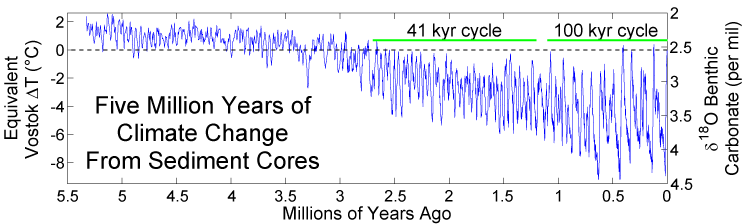
\includegraphics[width=0.7\hsize]{chapters/1/FiveMyrClimateChange.png}
\caption{Temperaturgeschichte der Erde aus 
\cite{skript:geologictemperaturerecord}
\label{skript:history:temperatur}}
\end{figure}%
Die Temperaturgeschichte der Erde konnte mit beachtlicher
Genauigkeit rekonstruiert werden.
Möglich ist dies, weil zum Beispiel die chemische Zusammensetzung sich
auch in der chemischen Zusammensetzung der Sedimente niederschlägt.
Die chemische Zusammensetzung wiederum erlaubt Rückschlüsse über das
Ausmass des Treibhauseffektes und damit der zu erwartenden Mitteltemperatur.
Es stellt sich heraus, dass die Temperatur sich auch auf das
Isotopenverhältnis von $\mathstrut^{16}\text{O}$ und
$\mathstrut^{18}\text{O}$ auswirkt, welches in den in Kalkschalen von
Foraminiferen
\index{Foraminiferen}%
aufgezeichnet wird.
In der jüngeren Erdgeschichte, etwa seit dem Kambrium, lässt sich aus
\index{Kambrium}%
den gefundenen Ablagerungen sowie aus Fossilien die Bewegung der
Kontinentalplatten und das dort herrschende Klima rekonstruieren.

Die zu entwickelnden Modelle für das Erdklima müssen konsistent sein
mit der Klimageschichte.
Zum Beispiel gibt es Hinweise, dass vor etwa 700 Milliarden Jahren die
Erde zeitweise sehr stark vereist war, es gibt sogar die Hypothese des
Snowball Earth welche besagt, dass die Erde zeitweise vollständig
\index{Snowball Earth}%
vereist war.
Wenn dem so ist, dann müssten Klimamodelle ebenfalls einen möglichen
stabilen Zustand
vorhersagen, bei dem die globale Mitteltemperatur deutlich tiefer ist.
Dies beobachtet man tatsächlich, schon die einfachen
Strahlungsbilanzmodelle in Abschnitt~\ref{skript:section:budyko}
haben ein stabiles Gleichgewicht bei sehr tiefer Temperatur.

In jüngerer Zeit stehen natürlich viel detailliertere Aufzeichnung der
Klimaentwicklung zur Verfügung, die zum Beispiel in Jahrringen von Bäumen
oder Bohrkernen aus dem Eis der Antarktis oder aus Grönland ablesbar sind.
In historischer Zeit stehen sogar direkte Messungen der chemischen
Zusammensetzung der Atmosphäre zur Verfügung.
Zum Beispiel wird die $\text{CO}_2$-Konzentration am Mauna Loa seit den 
Fünfzigerjahren gemessen.
Die Daten sind konsistent mit ähnlichen Messungen am Südpol.
Ebenso werden seit dem 19.~Jahrhundert detaillierte Aufzeichnungen
über die Wetterentwicklung an zahllosen Wetterstationen in der ganzen
Welt geführt.
In jüngster Zeit haben Satelliten
detaillierte Temperatur-Messungen der Erdoberfläche
ermöglicht.

Dieser umfassende Datensatz erlaubt heute, detaillierte Modelle
grosser Zuverlässigkeit zu erstellen, die selbst für längere Zeitintervalle
genaue Prognosen ermöglichen.
Es steht natürlich ausser Diskussion, dass im Rahmen dieses Seminars
ein solches Modell entwickelt werden könnte.
Es sollte aber mindestens möglich sein, durch statistische Analyse der
jüngsten Klimageschichte mit sehr geringer Irrtumswahrscheinlichkeit
nachzuweisen, dass sich das Klima tatsächlich verändert hat, wie es
in Kapitel~\ref{chapter:extrem} durchgeführt wird.

Als Entscheidungsgrundlage für Massnahmen zur Milderung der Auswirkungen
des Klimawandels ist ein solch detailliertes Modell nicht unbedingt notwendig.
Eine starke Korrelation zum Beispiel zwischen der $\text{CO}_2$-Konzentration
und der globalen Mitteltemperatur, wie wir sie aus den Messungen der
jüngsten Vergangenheit ablesen können und wie sie das später zu entwickelnde
Bilanzmodell oder das Budyko-Modell vorhersagen.







